\pagebreak
\section{Appendix}

\subsection{Implementation Details}
We begin by pretraining the source task model, $f_S$, using the task loss on the labeled source data. Next, we perform pixel-level adaptation using our image space GAN losses together with semantic consistency and cycle consistency losses. This yeilds learned parameters for the image transformations, $\StoT$ and $\TtoS$, image discriminators, $D_S$ and $D_T$, as well as an initial setting of the task model, $f_T$, which is trained using pixel transformed source images and the corresponding source pixel labels. Finally, we perform feature space adpatation in order to update the target semantic model, $f_T$, to have features which are aligned between the source images mapped into target style and the real target images. During this phase, we learn the feature discriminator, $D_\text{feat}$ and use this to guide the representation update to $f_T$. In general, our method could also perform phases 2 and 3 simultaneously, but this would require more GPU memory then available at the time of these experiments. 

For all feature space adaptation we equally weight the generator and discriminator losses. We only update the generator when the discriminator accuracy is above 60\% over the last batch (digits) or last 100 iterations (semantic segmentation) -- this reduces the potential for volatile training. If after an epoch (entire pass over dataset) no suitable discriminator is found, the feature adaptation stops, otherwise it continues until max iterations are reached. 



\subsubsection{Digit Experiments}
\label{sec:digit-details}
\begin{figure}
	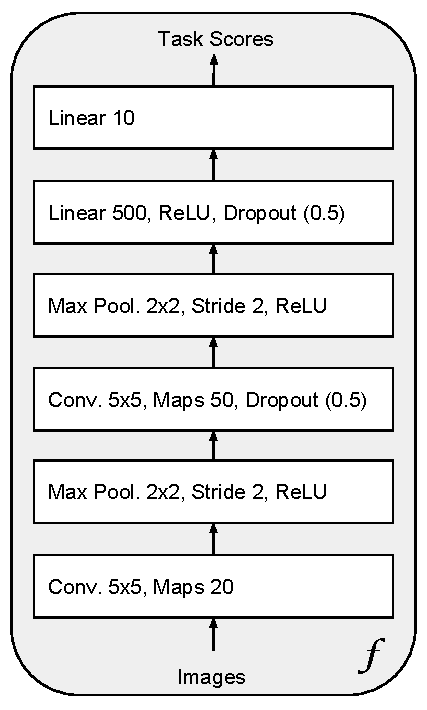
\includegraphics[width=.24\linewidth]{figs/digit_task_net.pdf}
	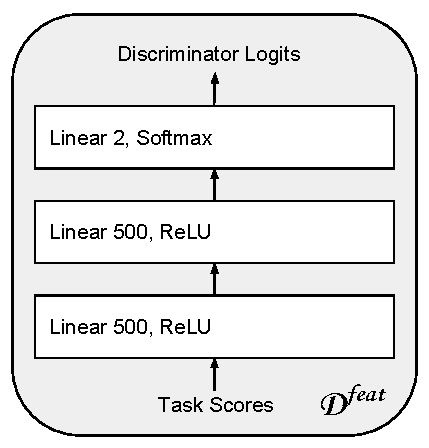
\includegraphics[width=.24\linewidth]{figs/digit_feat_discrim.pdf}
	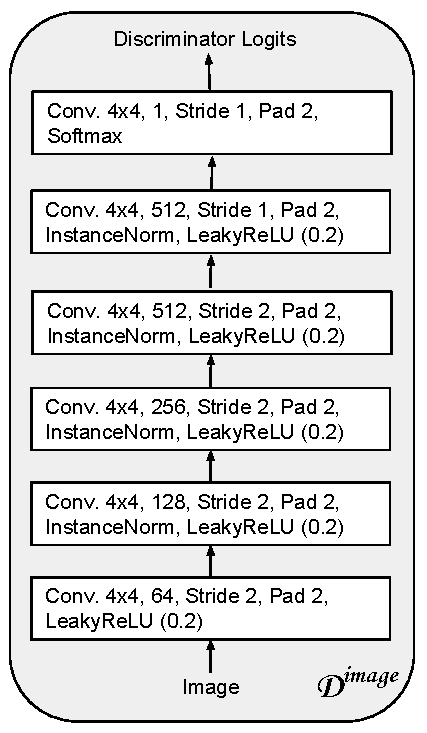
\includegraphics[width=.24\linewidth]{figs/digit_image_discrim.pdf}
	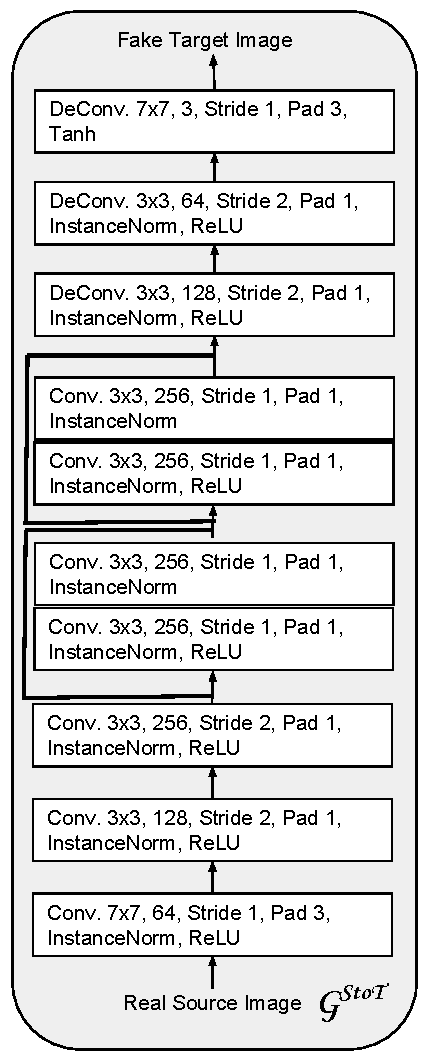
\includegraphics[width=.24\linewidth]{figs/digit_generator.pdf}
	\caption{Network architectures used for digit experiments. We show here the task net ($f$), discriminator for feature level adaptation ($D^{feat}$), discriminator for image level adaptation ($D^{image}$), and generator for source to target ($G$) -- same network used for target to source.}
	\label{fig:digit_nets}
\end{figure}
For all digit experiments we use a variant of the LeNet architecture as the task net (Figure~\ref{fig:digit_nets} \textit{left}). Our feature discriminator network consists of 3 fully connected layers (Figure~\ref{fig:digit_nets} \textit{mid left}). The image discriminator network consists of 6 convolutional layers culminating in a single value per pixel (Figure~\ref{fig:digit_nets} \textit{mid right}). Finally, to generate one image domain from another we use a multilayer network which consists of convolution layers followed by two residual blocks and then deconvolution layers (Figure~\ref{fig:digit_nets} \textit{right}). 
All stages are trained using the Adam optimizer. 

\paragraph{Hyperparameters.} For training the source task net model, we use learning rate 1e-4 and train for 100 epochs over the data with batch size 128. For feature space adaptation we use learning rate 1e-5 and train for max 200 epochs over the data. For pixel space adaptation we train our generators and discriminators with equal weighting on all losses, use batch size 100, learning rate 2e-4 (default from CycleGAN), and trained for 50 epochs. We ran each experiment 4 times and report the average and standard error across the runs.




\subsubsection{Semantic Segmentation}
\label{sec:ss-details}


\begin{figure}[h]
	\centerline{
  \setlength{\tabcolsep}{2.0pt}
  \begin{tabular}{cc cc}
    %\toprule
    %\textbf{GTA5}  & \textbf{GTA5 $\rightarrow$ Cityscapes} & \textbf{Cityscapes} & \textbf{Cityscapes $\rightarrow$ GTA5}\\
	%\midrule
%    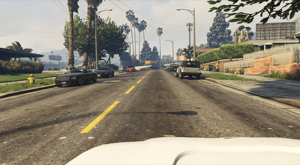
\includegraphics[width=\myw, height=\myh]{figs/gta-cityscapes/gta-00086-fs8.png} &
%    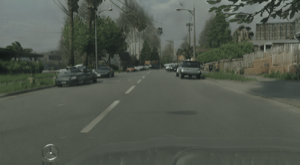
\includegraphics[width=\myw, height=\myh]{figs/gta-cityscapes/fake-cityscapes-00086-fs8.png} &
%    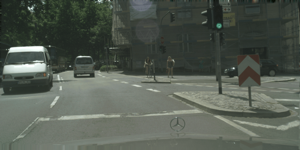
\includegraphics[width=\myw, height=\myh]{figs/gta-cityscapes/cityscapes-00086-fs8.png} &
%    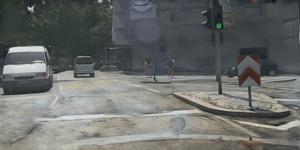
\includegraphics[width=\myw, height=\myh]{figs/gta-cityscapes/fake-gta-00086-fs8.png}
%    \\
%    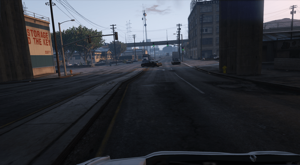
\includegraphics[width=\myw, height=\myh]{figs/gta-cityscapes/gta-00220-fs8.png} &
%    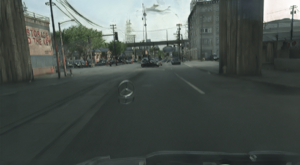
\includegraphics[width=\myw, height=\myh]{figs/gta-cityscapes/fake-cityscapes-00220-fs8.png} &
%    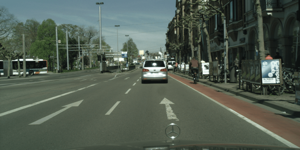
\includegraphics[width=\myw, height=\myh]{figs/gta-cityscapes/cityscapes-00220-fs8.png} &
%    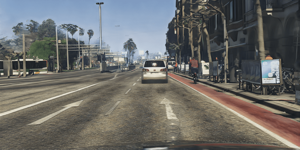
\includegraphics[width=\myw, height=\myh]{figs/gta-cityscapes/fake-gta-00220-fs8.png}
%   \\
    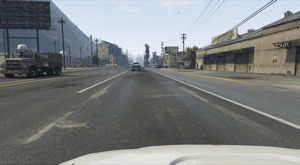
\includegraphics[width=\myw, height=\myh]{figs/gta-cityscapes/gta-00702-fs8.png} &
    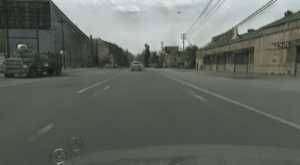
\includegraphics[width=\myw, height=\myh]{figs/gta-cityscapes/fake-cityscapes-00702-fs8.png} &
    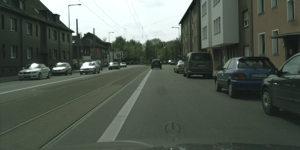
\includegraphics[width=\myw, height=\myh]{figs/gta-cityscapes/cityscapes-00702-fs8.png} &
    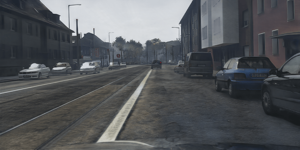
\includegraphics[width=\myw, height=\myh]{figs/gta-cityscapes/fake-gta-00702-fs8.png}
   \\
    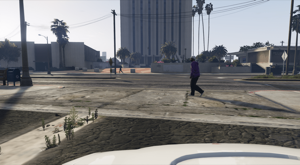
\includegraphics[width=\myw, height=\myh]{figs/gta-cityscapes/gta-01490-fs8.png} &
    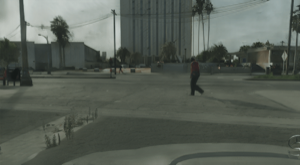
\includegraphics[width=\myw, height=\myh]{figs/gta-cityscapes/fake-cityscapes-01490-fs8.png} &
    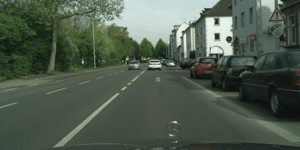
\includegraphics[width=\myw, height=\myh]{figs/gta-cityscapes/cityscapes-01490-fs8.png} &
    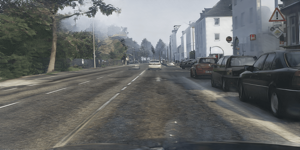
\includegraphics[width=\myw, height=\myh]{figs/gta-cityscapes/fake-gta-01490-fs8.png}
   \\
    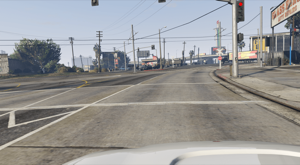
\includegraphics[width=\myw, height=\myh]{figs/gta-cityscapes/gta-01946-fs8.png} &
    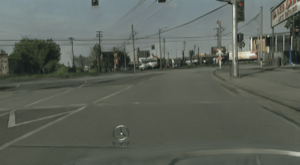
\includegraphics[width=\myw, height=\myh]{figs/gta-cityscapes/fake-cityscapes-01946-fs8.png} &
    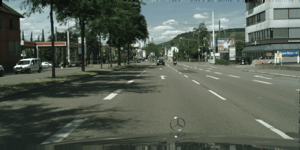
\includegraphics[width=\myw, height=\myh]{figs/gta-cityscapes/cityscapes-01946-fs8.png} &
    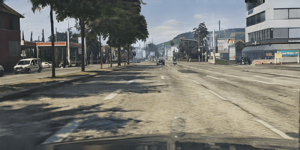
\includegraphics[width=\myw, height=\myh]{figs/gta-cityscapes/fake-gta-01946-fs8.png}
   \\
    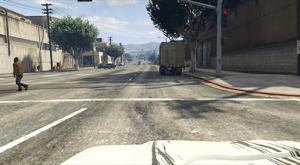
\includegraphics[width=\myw, height=\myh]{figs/gta-cityscapes/gta-02212-fs8.png} &
    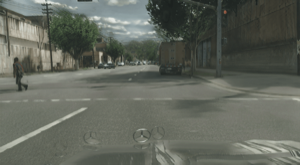
\includegraphics[width=\myw, height=\myh]{figs/gta-cityscapes/fake-cityscapes-02212-fs8.png} &
    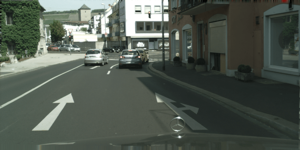
\includegraphics[width=\myw, height=\myh]{figs/gta-cityscapes/cityscapes-02212-fs8.png} &
    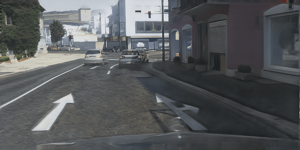
\includegraphics[width=\myw, height=\myh]{figs/gta-cityscapes/fake-gta-02212-fs8.png}
   \\
    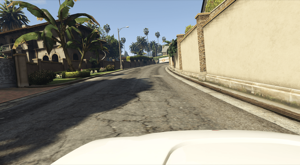
\includegraphics[width=\myw, height=\myh]{figs/gta-cityscapes/gta-03655-fs8.png} &
    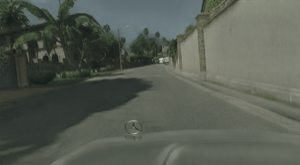
\includegraphics[width=\myw, height=\myh]{figs/gta-cityscapes/fake-cityscapes-03655-fs8.png} &
    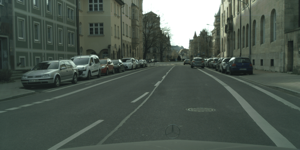
\includegraphics[width=\myw, height=\myh]{figs/gta-cityscapes/cityscapes-03655-fs8.png} &
    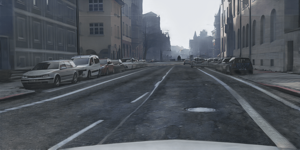
\includegraphics[width=\myw, height=\myh]{figs/gta-cityscapes/fake-gta-03655-fs8.png}
   \\
    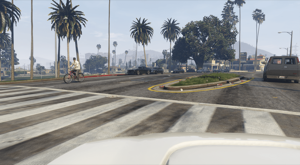
\includegraphics[width=\myw, height=\myh]{figs/gta-cityscapes/gta-02612-fs8.png} &
    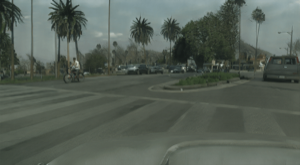
\includegraphics[width=\myw, height=\myh]{figs/gta-cityscapes/fake-cityscapes-02612-fs8.png} &
    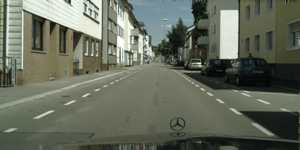
\includegraphics[width=\myw, height=\myh]{figs/gta-cityscapes/cityscapes-02612-fs8.png} &
    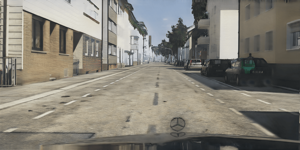
\includegraphics[width=\myw, height=\myh]{figs/gta-cityscapes/fake-gta-02612-fs8.png}
   \\
   (a) GTA5 & (b) GTA5 $\rightarrow$ Cityscapes & (c) CityScapes & (d) CityScapes $\rightarrow$ GTA5
   %\bottomrule
  \end{tabular}
  }
  \caption{%\small
  \textbf{GTA5 to CityScapes Image Translation.} Example images from the GTA5 (a) and Cityscapes (c) datasets, alongside their image-space conversions to the opposite domain, (b) and (d), respectively. Our model achieves highly realistic domain conversions.}
  \label{fig:gta-cityscapes-appendix}
\end{figure}

We experiment with both the VGG16-FCN8s~\cite{long_cvpr15} architecture as well as the DRN-26~\cite{drn} architecture. 
For FCN8s, we train our source semantic segmentation model for 100k iterations using SGD with learning rate 1e-3 and momentum 0.9.
For the DRN-26 architecture, we train our source semantic segmentation model for 115K iterations using SGD with learning rate 1e-3 and momentum 0.9. We use a crop size of 600x600 and a batch size of 8 for this training. 
For cycle-consistent image level adaptation, we followed the network architecture and hyperparameters of CycleGAN\citep{zhu_arxiv17}.
All images were resized to have width of 1024 pixels while keeping the aspect ratio, and the training was performed with randomly cropped patches of size 400 by 400. Also, due to large size of the dataset, we trained only 20 epochs.
For feature level adaptation, we train using SGD with momentum, 0.99, and learning rate 1e-5. We weight the representation loss ten times less than the discriminator loss as a convienience since otherwise the discriminator did not learn a suitable model within a single epoch. Then the segmentation model was trained separately using the adapted source images and the ground truth labels of the source data. Due to memory limitations we can only include a single source and single target image at a time (crops of size 768x768), this small batch is one of the main reasons for using a high momentum parameter.

\subsection{Comparison to \citet{shrivastava_cvpr17} for Semantic Segmentation}
We illustrate the performance of a recent pixel level adaptation approach proposed by \citet{shrivastava_cvpr17} on our semantic segmentation data -- GTA to Cityscapes. These images are significantly larger and more complex than those shown in the experiments in the original paper. We show image to image translation results under three different settings of the model hyperparameter, $\lambda$, which controls the tradeoff between the reconstruction loss and the visual style loss. When $\lambda=10$ (Figure~\ref{fig:shrivastava} \textit{right}), the resulting image converges to a near replica of the original image, thus preserving content but lacking the correct target style. When $\lambda=1$ or $\lambda=2.5$ (Figure~\ref{fig:shrivastava} \textit{left}), the results lack any consistent semantics making it difficult to perceive the style of the transformed image. Thus, the resulting performance for this model is 11.6 mIoU for FCN8s with VGG, well below the performance of the corresponding source model of 17.9 mIoU. 
\begin{figure}
	\centering
	\begin{tabular}{ccc}
		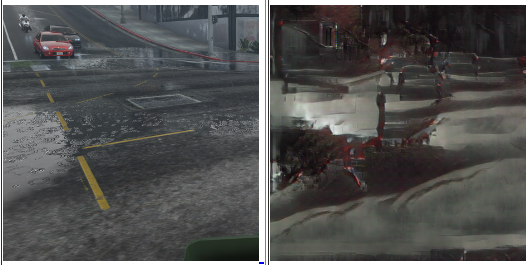
\includegraphics[width=.32\linewidth]{figs/apple-paper-results/lambda1_ep10.png} &
		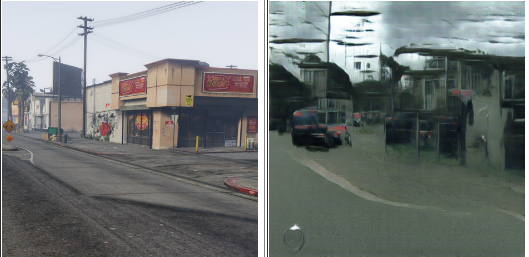
\includegraphics[width=.32\linewidth]{figs/apple-paper-results/lambda2p5_ep10.png}&
		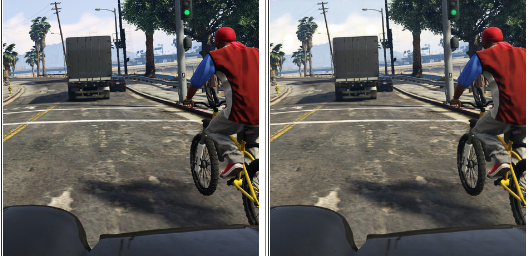
\includegraphics[width=.32\linewidth]{figs/apple-paper-results/lambda10_ep10.png}\\
		(a) $\lambda = 1$ & (b) $\lambda = 2.5$ & (c) $\lambda = 10$	
\end{tabular}

\caption{Image transformation results from \citet{shrivastava_cvpr17} applied to GTA to CityScapes transformation. We demonstrate results using three different settings for $\lambda$.}
\label{fig:shrivastava}
\end{figure}

\subsection{Experiment Analysis}
To understand the types of mistakes which are improved upon and those which still persist after adaptation, we present the confusion matricies before and after our approach for the digit experiment of SVHN to MNIST (Figure~\ref{fig:digit_err}). Before adaptation we see common confusions are 0s with 2s, 4s, and 7s. 6 with 4, 8 with 3, and 9 with 4. After adaptation all errors are reduced, but we still find that 7s are confused with 1s and 0s with 2s. These errors make some sense as with hand written digits, these digits sometimes resemble one another. It remains an open question to produce a model which may overcome these types of errors between highly similar classes.  
\begin{figure}
	\centering
	\begin{tabular}{cc}
		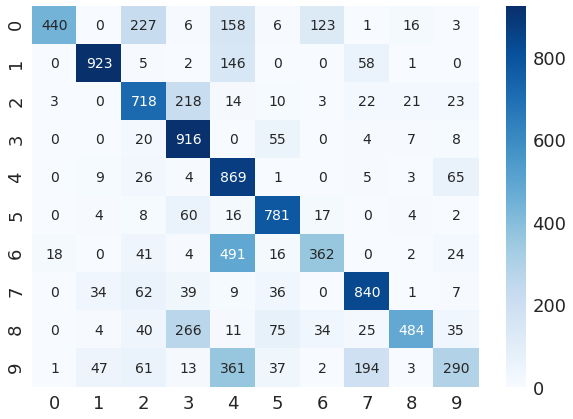
\includegraphics[width=.45\linewidth]{figs/confusionmat_svhn2mnist_src} &
		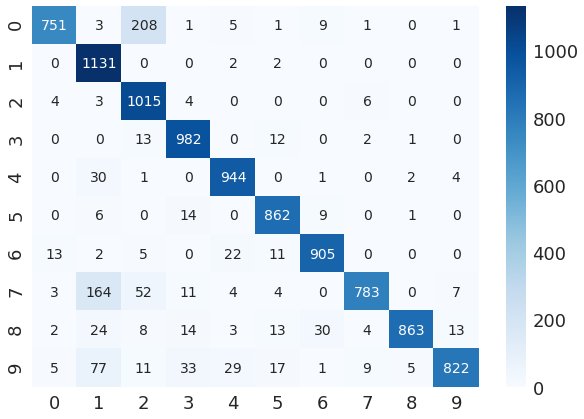
\includegraphics[width=.45\linewidth]{figs/confusionmat_svhn2mnist_cycada}\\
		(a) Source only Model & (b) CyCADA model
	\end{tabular}	
	\caption{Confusion matricies for SVHN $\rightarrow$ MNIST experiment. }
	\label{fig:digit_err}
\end{figure}

